\def\linkdethi{} %Đường link cần dẫn tới
\anmaQR
%%%%%%%%%%%%%%%%%%%%%%%%
\def\toanlop{12}
\def\thoigian{90}
\def\namhoc{2025 - 2026}
\begin{dethi}
	{Bộ GD\&ĐT}
	{VTED ft KING EDU}
	{TDMT14}
	{Đề thi thử THPTQG 2026}
\end{dethi}
\caulc
\Opensolutionfile{ans}[ans/ansTN-Dung]
%%%%=============EX_1=============%%%
%\begin{ex}%[1D6H4-3]%[TDMT14]%[Mui Doan]
%	Tập nghiệm của bất phương trình $\log_{0{,}7}(x-2)>0$ là
%	\choice
%	{$(3;+\infty)$}
%	{$(-\infty;3)$}
%	{\True $(2;3)$}
%	{$(3;4)$}
%	\loigiai{
%		Điều kiện xác định $x-2>0 \Leftrightarrow x>2$.\\
%		Vì cơ số $a=0{,}7 \in (0;1)$ nên bất phương trình đã cho tương đương với
%		\begin{align*}
%			x-2 < 0{,}7^0 \Leftrightarrow x-2 < 1 \Leftrightarrow x < 3.
%		\end{align*}
%		Kết hợp với điều kiện xác định, ta được $2 < x < 3$.\\
%		Vậy tập nghiệm của bất phương trình là $S = (2;3)$.
%	}
%\end{ex}
%%%%=============================%%%
%
%%%%=============EX_2=============%%%
%\begin{ex}%[1H8H7-3]%[TDMT14]%[Huỳnh Trí Thiện]
%	\immini[thm]{Cho hình chóp tam giác $S.ABC$ có đáy là tam giác đều cạnh $a$. Cạnh bên $SA$ vuông góc với đáy $(ABC)$ và có $SA=2a$. Thể tích khối chóp $S.ABC$ bằng
%		\choice
%		{$\dfrac{a^3\sqrt{3}}{2}$}
%		{\True $\dfrac{a^3\sqrt{3}}{6}$}
%		{$\dfrac{a^3\sqrt{3}}{12}$}
%		{$\dfrac{a^3\sqrt{6}}{12}$}}{
%		\begin{tikzpicture}[declare function={a=3; b=0.5*a; h=0.65*a;},line join=round,line cap=round,>=stealth,font=\footnotesize]
%			\path (0,0) coordinate (A)
%			(a,0) coordinate (C)
%			(-45:b) coordinate (B)
%			($(A)+(0,h)$) coordinate (S);
%			\foreach \x/\y/\z in {B/A/S,C/A/S}{
%				\path pic[draw,angle radius=5pt]{right angle=\x--\y--\z};
%			}
%			\draw[dashed] (A)--(C);
%			\draw (S)--(B)
%			(S)--(A)--(B)--(C)--cycle;
%			\foreach \x/\goc in {S/90,A/190,B/-90,C/0}
%			\fill (\x) circle (1pt) node[shift={(\goc:7pt)}]{$\x$};
%		\end{tikzpicture}
%	}
%	\loigiai{
%		Vì tam giác $ABC$ là tam giác đều cạnh $a$ nên diện tích đáy là $S_{\triangle ABC} = \dfrac{a^2\sqrt{3}}{4}$.\\
%		Thể tích khối chóp $S.ABC$ là
%		\begin{align*}
%			V = \dfrac{1}{3} \cdot S_{\triangle ABC} \cdot SA = \dfrac{1}{3} \cdot \dfrac{a^2\sqrt{3}}{4} \cdot 2a = \dfrac{a^3\sqrt{3}}{6}.
%		\end{align*}
%		Vậy thể tích khối chóp cần tìm là $\dfrac{a^3\sqrt{3}}{6}$.
%	}
%\end{ex}
%%%%=============================%%%
%
%%%%=============EX_3=============%%%
%\begin{ex}%[1D2H2-2]%[TDMT14]%[Chu Hà]
%	Cho cấp số cộng $(u_n)$ có $u_1=1$ và $u_3=7$. Công sai của $(u_n)$ bằng
%	\choice
%	{$6$}
%	{\True $3$}
%	{$8$}
%	{$2$}
%	\loigiai{
%		Gọi $d$ là công sai của cấp số cộng $(u_n)$. Theo công thức số hạng tổng quát, ta có
%		\begin{align*}
%			u_3 = u_1 + 2d.
%		\end{align*}
%		Thay số vào ta được $7 = 1 + 2d \Leftrightarrow 2d = 6 \Leftrightarrow d = 3$.\\
%		Vậy công sai của cấp số cộng là $d=3$.
%	}
%\end{ex}
%%%%=============================%%%
%
%%%%=============EX_4=============%%%
%\begin{ex}%[1D6H4-5]%[TDMT14]%[Nguyễn Tấn Linh]
%	Số nghiệm nguyên của bất phương trình $\left(3+\sqrt{x-4}\right)\left(3\ln x - \ln^2 x\right) \ge 0$ là
%	\choice
%	{$20$}
%	{$7$}
%	{\True $17$}
%	{$4$}
%	\loigiai{
%		Điều kiện xác định $\heva{&x-4 \ge 0 \\ &x > 0} \Leftrightarrow x \ge 4$.\\
%		Với mọi $x \ge 4$, ta luôn có $3 + \sqrt{x-4} > 0$. \\
%		Do đó, bất phương trình đã cho tương đương với
%		\begin{align*}
%			3\ln x - \ln^2 x \ge 0 \Leftrightarrow \ln x (3 - \ln x) \ge 0 \Leftrightarrow 0 \le \ln x \le 3 \Leftrightarrow 1 \le x \le \mathrm{e}^3.
%		\end{align*}
%		Kết hợp với điều kiện xác định, ta được $4 \le x \le \mathrm{e}^3$.\\
%		Vì $x \in \mathbb{Z}$ và $\mathrm{e}^3 \approx 20{,}08$ nên $x \in \{4; 5; 6; \dots; 20\}$.\\
%		Vậy bất phương trình có $20 - 4 + 1 = 17$ nghiệm nguyên.
%	}
%\end{ex}
%%%%=============================%%%
%
%%%%=============EX_5=============%%%
%\begin{ex}%[2D4H1-3]%[TDMT14]%[Phạm Hải Dương]
%	Họ nguyên hàm của hàm số $f(x) = \dfrac{2}{\sin^2 x}$, với $x \neq k\pi$ ($k \in \mathbb{Z}$), là
%	\choice
%	{$-\tan x + C$}
%	{$-\cot x + C$}
%	{$-2\tan x + C$}
%	{\True $-2\cot x + C$}
%	\loigiai{
%		Ta có họ nguyên hàm của hàm số $f(x) = \dfrac{2}{\sin^2 x}$ là
%		\begin{align*}
%			\displaystyle\int \dfrac{2}{\sin^2 x} \mathrm{d}x = 2 \int \dfrac{1}{\sin^2 x} \mathrm{d}x = 2(-\cot x) + C = -2\cot x + C.
%		\end{align*}
%	}
%\end{ex}
%%%%=============================%%%
%
%%%%=============EX_6=============%%%
%\begin{ex}%[2D1N2-2]%[TDMT14]%[Nguyễn Sơn Thành]
%	\immini[thm]{Cho đồ thị hàm số $y=f(x)$ như hình vẽ bên dưới. Hỏi hàm số $f(x)$ có tất cả bao nhiêu điểm cực trị?
%		\choice
%		{\True $4$}
%		{$5$}
%		{$2$}
%		{$3$}
%	}{	
%		\begin{tikzpicture}[scale=0.6,>=stealth,font=\footnotesize,line join=round,line cap=round]
%			\draw[->] (-5,0)--(4,0) node[shift={(-100:7pt)},font=\scriptsize]{$x$};
%			\draw[->] (0,-1.5)--(0,4) node[shift={(180:7pt)},font=\scriptsize]{$y$};
%			\fill (0,0) circle (1.2pt) node[below left,font=\scriptsize] {$O$};
%			\draw (-4,-1)--(-2.5,3)--(-1,-0.5) plot[smooth,tension=0.6] coordinates {(-1,-0.5) (0.7,2.5) (2,0) (3.2,3.5)};
%			\node at (3,3.5) [font=\scriptsize,right]{$f(x)$};
%		\end{tikzpicture}
%	}
%	\loigiai{
%		Dựa vào đồ thị hàm số $y=f(x)$, ta thấy hàm số đổi chiều biến thiên $4$ lần (từ đồng biến sang nghịch biến và ngược lại). \\
%		Cụ thể, đồ thị có $2$ điểm cực đại (đỉnh nhô lên) và $2$ điểm cực tiểu (đáy lõm xuống).\\
%		Vậy hàm số có tất cả $4$ điểm cực trị.
%	}
%\end{ex}
%%%%=============================%%%
%
%%%%=============EX_7=============%%%
%\begin{ex}%[2H2N2-4]%[TDMT14]%[Bồ Văn Hậu]
%	Trong không gian $Oxyz$, cho hai vectơ $\overrightarrow{u}=(-3;1;-1)$ và $\overrightarrow{v}=(1;0;5)$. Tích vô hướng của hai vectơ $\overrightarrow{u}$ và $\overrightarrow{v}$ bằng
%	\choice
%	{\True $-8$}
%	{$8$}
%	{$3$}
%	{$-3$}
%	\loigiai{
%		Áp dụng công thức tính tích vô hướng theo tọa độ, ta có
%		\begin{align*}
%			\overrightarrow{u}\cdot \overrightarrow{v} = (-3)\cdot 1 + 1\cdot 0 + (-1)\cdot 5 = -3 + 0 - 5 = -8.
%		\end{align*}
%	}
%\end{ex}
%%%%=============================%%%
%
%%%%=============EX_8=============%%%
%\begin{ex}%[2D4H2-1]%[TDMT14]%[Lê Phúc]
%	Cho biết $\displaystyle\int\limits^1_0 f(x) \mathrm{\,d}x=3$ và $\displaystyle\int\limits^2_1 2f(x) \mathrm{\,d}x=4$. Giá trị $\displaystyle\int\limits^2_0 f(x) \mathrm{\,d}x$ bằng
%	\choice
%	{$7$}
%	{$12$}
%	{\True $5$}
%	{$-1$}
%	\loigiai{
%		Áp dụng tính chất của tích phân, ta có
%		\begin{align*}
%			\displaystyle\int\limits^2_1 2f(x) \mathrm{\,d}x=4 \Leftrightarrow 2\displaystyle\int\limits^2_1 f(x) \mathrm{\,d}x=4 \Leftrightarrow \displaystyle\int\limits^2_1 f(x) \mathrm{\,d}x=2.
%		\end{align*}
%		Theo tính chất chèn cận của tích phân, ta có
%		\begin{align*}
%			\displaystyle\int\limits^2_0 f(x) \mathrm{\,d}x = \displaystyle\int\limits^1_0 f(x) \mathrm{\,d}x + \displaystyle\int\limits^2_1 f(x) \mathrm{\,d}x = 3 + 2 = 5.
%		\end{align*}
%	}
%\end{ex}
%%%%=============================%%%
%
%%%%=============EX_9=============%%%
%\begin{ex}%[2H5N3-2]%[TDMT14]%[Trần Văn Thiện]
%	Trong không gian $Oxyz$, cho mặt cầu $(S)\colon x^2+y^2+z^2-4x-2=0$. Bán kính của mặt cầu $(S)$ là
%	\choice
%	{$6$}
%	{$2$}
%	{$2\sqrt{2}$}
%	{\True $\sqrt{6}$}
%	\loigiai{
%		Mặt cầu $(S)$ có phương trình $x^2+y^2+z^2-4x-2=0$.\\
%		Ta biến đổi về phương trình dạng chuẩn
%		\begin{align*}
%			(x^2-4x+4) + y^2 + z^2 = 2 + 4 \Leftrightarrow (x-2)^2+y^2+z^2=6.
%		\end{align*}
%		Suy ra bán kính của mặt cầu $(S)$ là $R = \sqrt{6}$.
%	}
%\end{ex}
%%%%=============================%%%
%
%%%%=============EX_10=============%%%
%\begin{ex}%[2D1H3-2]%[TDMT14]%[Đình Nguyên]
%	Giá trị nhỏ nhất của hàm số $f(x) = x^3 - 6x$ trên khoảng $(0; +\infty)$ bằng
%	\choice
%	{$0$}
%	{$4\sqrt{2}$}
%	{\True $-4\sqrt{2}$}
%	{$-2\sqrt{2}$}
%	\loigiai{
%		Xét hàm số $f(x) = x^3 - 6x$ trên khoảng $(0; +\infty)$.\\
%		Ta có $f'(x) = 3x^2 - 6$.\\
%		Khi đó $f'(x) = 0 \Leftrightarrow 3x^2 - 6 = 0 \Leftrightarrow x^2 = 2 \Leftrightarrow \hoac{&x = \sqrt{2}\in (0; +\infty)\\&x = -\sqrt{2}\notin (0; +\infty).}$\\
%		Bảng biến thiên
%		\begin{center}
%			\begin{tikzpicture}[font=\normalsize,t style/.style={style=solid}]
%				\tkzTabInit[nocadre=false,lgt=1.2,espcl=2.5,deltacl=0.5]
%				{$x$/0.75,$f'(x)$/0.75,$f(x)$/3}
%				{$0$,$\sqrt{2}$,$+\infty$}
%				\tkzTabLine{,-,0,+}
%				\path
%				($(N13)!0.6!(N12)$) node (A1){$0$}
%				($(N23)!0.1!(N22)$) node (A2){$-4\sqrt{2}$}
%				($(N33)!0.8!(N32)$) node (A3){$+\infty$};
%				\foreach \x/\y in {A1/A2,A2/A3}{
%					\draw[-stealth] (\x)--(\y);
%				}
%			\end{tikzpicture}
%		\end{center}
%		Dựa vào bảng biến thiên, ta thấy hàm số đạt giá trị nhỏ nhất tại $x = \sqrt{2}$.\\
%		Vậy $\displaystyle\min\limits_{(0; +\infty)} f(x) = f\left(\sqrt{2}\right) = \left(\sqrt{2}\right)^3 - 6\sqrt{2} = 2\sqrt{2} - 6\sqrt{2} = -4\sqrt{2}$.
%	}
%\end{ex}
%%%%=============================%%%
%
%%%%=============EX_11=============%%%
%\begin{ex}%[1D5V1-3]%[TDMT14]%[Huỳnh Quốc Đạt]
%	Cho hai mẫu số liệu ghép nhóm $M_1$, $M_2$ với bảng tần số ghép nhóm như sau
%	\begin{center}
%		\begin{tabular}{|c|c|c|c|c|c|c|c|}
%			\hline
%			\multirow{2}{*}{$M_1$} & Nhóm & $[8;10)$ & $[10;12)$ & $[12;14)$ & $[14;16)$ & $[16;18)$ & $[18;20)$ \\
%			\cline{2-8}
%			& Tần số & $6$ & $6$ & $8$ & $4$ & $6$ & $7$ \\
%			\hline
%			\multirow{2}{*}{$M_2$} & Nhóm & $[8;10)$ & $[10;12)$ & $[12;14)$ & $[14;16)$ & $[16;18)$ & $[18;20)$ \\
%			\cline{2-8}
%			& Tần số & $6$ & $6$ & $8$ & $4$ & $6$ & $a$ \\
%			\hline
%		\end{tabular}
%	\end{center}
%	Hỏi có tất cả bao nhiêu giá trị nguyên nhỏ hơn $20$ của $a$ để số trung bình cộng của mẫu số liệu $M_2$ lớn hơn của mẫu số liệu $M_1$?
%	\choice
%	{$11$}
%	{\True $12$}
%	{$13$}
%	{$6$}
%	\loigiai{
%		Ta tính các giá trị đại diện cho mỗi nhóm lần lượt là $9$; $11$; $13$; $15$; $17$; $19$.\\
%		Xét mẫu số liệu $M_1$:\\
%		Cỡ mẫu là $N_1 = 6+6+8+4+6+7 = 37$.\\
%		Số trung bình của nhóm $M_1$ là
%		\begin{align*}
%			\overline{x}_1 = \dfrac{9\cdot 6 + 11\cdot 6 + 13\cdot 8 + 15\cdot 4 + 17\cdot 6 + 19\cdot 7}{37} = \dfrac{54+66+104+60+102+133}{37} = \dfrac{519}{37}.
%		\end{align*}
%		Xét mẫu số liệu $M_2$:\\
%		Cỡ mẫu là $N_2 = 6+6+8+4+6+a = 30+a$.\\
%		Số trung bình của nhóm $M_2$ là
%		\begin{align*}
%			\overline{x}_2 = \dfrac{9\cdot 6 + 11\cdot 6 + 13\cdot 8 + 15\cdot 4 + 17\cdot 6 + 19\cdot a}{30+a} = \dfrac{386+19a}{30+a}.
%		\end{align*}
%		Yêu cầu bài toán $\overline{x}_2 > \overline{x}_1 \Leftrightarrow \dfrac{386+19a}{30+a} > \dfrac{519}{37}$.\\
%		Vì $a$ là tần số nên $a \ge 0$, do đó $30+a > 0$. Khi đó
%		\begin{align*}
%			& 37(386+19a) > 519(30+a) \\
%			\Leftrightarrow \ & 14\,282 + 703a > 15\,570 + 519a \\
%			\Leftrightarrow \ & 184a > 1\,288 \\
%			\Leftrightarrow \ & a > 7.
%		\end{align*}
%		Vì $a$ là số nguyên và $a < 20$ nên $a \in \{8; 9; 10; \dots; 19\}$.\\
%		Vậy có tất cả $19 - 8 + 1 = 12$ giá trị $a$ thoả mãn yêu cầu bài toán.
%	}
%\end{ex}
%%%%=============================%%%
%
%%%%=============EX_12=============%%%
%\begin{ex}%[2H2H2-4]%[TDMZW04]%[Nguyễn Trí Minh Tuấn]
%	Cho tứ diện đều $ABCD$ có cạnh bằng $6$. Giá trị của biểu thức $\left(\overrightarrow{AB}+\overrightarrow{AC}\right)\cdot \overrightarrow{AD}$ bằng
%	\choice
%	{\True $36$}
%	{$0$}
%	{$18\sqrt{3}$}
%	{$72$}
%	\loigiai{
%		\immini{
%			Vì $ABCD$ là tứ diện đều có cạnh bằng $6$ nên $AB=AC=AD=6$.\\
%			Lại có các mặt $\triangle ABD$ và $\triangle ACD$ là các tam giác đều nên $\widehat{BAD}=60^\circ$ và $\widehat{CAD}=60^\circ$.\\
%			Xét các tích vô hướng
%			\begin{align*}
%				\overrightarrow{AB}\cdot \overrightarrow{AD} &= AB \cdot AD \cdot \cos\widehat{BAD} = 6 \cdot 6 \cdot \cos 60^\circ = 18,\\
%				\overrightarrow{AC}\cdot \overrightarrow{AD} &= AC \cdot AD \cdot \cos\widehat{CAD} = 6 \cdot 6 \cdot \cos 60^\circ = 18.
%			\end{align*}
%		}{
%			\begin{tikzpicture}[scale=1,font=\footnotesize,line join=round,line cap=round,>=stealth,declare function={a=3; b=0.45*a; h=0.65*a;}]
%				\path (0,0) coordinate (B)
%				(a,0) coordinate (D)
%				(-45:b) coordinate (C)
%				($(B)!0.5!(C)$) coordinate (Dp)
%				($(D)!0.5!(C)$) coordinate (Bp)
%				(intersection of D--Dp and B--Bp) coordinate (O)
%				($(O)+(0,h)$) coordinate (A);
%				\path pic[draw,angle radius=3pt]{right angle=B--O--A};
%				\path pic[draw,angle radius=3pt]{right angle=Dp--O--A};
%				\draw[dashed] (C)--(O)
%				(B)--(O)
%				(A)--(O)--(D)
%				(B)--(D);
%				\draw (A)--(C)
%				(A)--(B)--(C)--(D)--cycle;
%				\foreach \x/\goc/\t in {A/90/A,B/190/B,C/-90/C,D/0/D,O/-30/O}{
%					\fill (\x) node[shift={(\goc:7pt)},font=\scriptsize]{$\t$} circle (1pt);
%				}
%			\end{tikzpicture}
%		}		
%		Khi đó, áp dụng tính chất phân phối của tích vô hướng ta có
%		\begin{align*}
%			\left(\overrightarrow{AB}+\overrightarrow{AC}\right)\cdot \overrightarrow{AD} = \overrightarrow{AB}\cdot \overrightarrow{AD} + \overrightarrow{AC}\cdot \overrightarrow{AD} = 18 + 18 = 36.
%		\end{align*}
%	}
%\end{ex}
%%%%=============================%%%
\Closesolutionfile{ans}

\cauds
\Opensolutionfile{ans}[ans/ansTN-DungSai]
%%%%=============EX_13=============%%%
%\begin{ex}%[2D1V1-4]%[TDMT14]%[Dương Công Tạo]
%	Cho hàm số $f(x) = 3^x - 2x-1$.
%	\choiceTF[t]
%	{$f'(x) = 3^x - 2$}
%	{$\min f(x) = -\dfrac{1}{3}$}
%	{$f(x)\ge 0\Leftrightarrow x\ge 1$}
%	{\True $\left[f(x)+2x+1\right]^2 \le 8x+1\Leftrightarrow 0\le x\le 1$}
%	\loigiai{
%		\begin{itemchoice}
%			\itemch Ta có $f(x) = 3^x - 2x-1$.\\ Suy ra $f'(x) = 3^x\cdot\ln 3 - 2$. 
%			\itemch Xét hàm số $f(x) = 3^x - 2x-1$.\\
%			Tập xác định $\mathscr{D}=\mathbb{R}$.\\
%			Ta có $f'(x)=0\Leftrightarrow 3^x\cdot\ln 3 - 2=0\Leftrightarrow x=\log_3\left(\dfrac{2}{\ln 3}\right)$.\\
%			Ta tiến hành lập bảng biến thiên của hàm số $f(x)$ như bên dưới
%			\begin{center}
%				\begin{tikzpicture}[>=stealth,line join=round,line cap=round,every node/.style={font=\scriptsize}]
%					\tkzTabInit[nocadre=false,lgt=1.5,espcl=3.5,deltacl=0.6]
%					{$x$/1.2,$f'(x)$/0.7,$f(x)$/3}
%					{$-\infty$,$\log_3\left(\dfrac{2}{\ln 3}\right)$,$+\infty$}
%					\tkzTabLine{,-,0,+,}
%					\path
%					([yshift=-8pt]N12) node (A1) {$+\infty$}
%					([yshift=8pt]N23) node (A2) {$\min f(x)$}
%					([yshift=-8pt]N32) node (A3) {$+\infty$};
%					\draw[-stealth] (A1) -- (A2);
%					\draw[-stealth] (A2) -- (A3);
%					\coordinate (V0) at ($(N11)!0.3!(N21)$);
%					\coordinate (V1) at ($(N21)!0.7!(N31)$);
%					\path ([yshift=0.6cm]V0) node (Z0) {$0$};
%					\path ([yshift=0.6cm]V1) node (Z1) {$1$};
%					\coordinate (P1) at ($(A1.center)!0.3!(A2.center)$);
%					\coordinate (P2) at ($(A2.center)!0.7!(A3.center)$);
%					\draw[dashed] ([yshift=-2pt]Z0.south) -- (P1);
%					\draw[dashed] ([yshift=-2pt]Z1.south) -- (P2);
%					\coordinate (H1) at ($(P1)!-0.15!(P2)$);
%					\coordinate (H2) at ($(P2)!-0.15!(P1)$);
%					\draw[red,thick] (H1) -- (H2) node[pos=0.7,above] {$y=0$};
%					\fill (P1) circle (1pt);
%					\fill (P2) circle (1pt);
%				\end{tikzpicture}
%			\end{center}
%			Từ bảng biến thiên, ta có $\min\limits_{\mathbb{R}}f(x)=f\left[\log_3\left(\dfrac{2}{\ln 3}\right)\right]=\dfrac{2}{\ln 3} - 2\log_3\left(\dfrac{2}{\ln 3}\right)-1$.
%			\itemch Dựa vào bảng biến thiên, ta có $f(x)\ge 0\Leftrightarrow \hoac{&x\le 0\\&x\ge 1.}$ 
%			\itemch Bất phương trình $\left[f(x)+2x+1\right]^2 \le 8x+1 \Leftrightarrow \left(3^x\right)^2 \le 8x+1 \Leftrightarrow 9^x \le 8x+1$.\\
%			Dựa vào bảng biến thiên của hàm số ta có $f(x) \le 0 \Leftrightarrow 3^x \le 2x+1 \Leftrightarrow 0 \le x \le 1$.\\
%			Khi đó ta sẽ có tổng quát $(1+a)^x \le ax+1 \Leftrightarrow 0 \le x \le 1$ với $a > 0$.\\
%			Áp dụng $\left(3^x\right)^2 \le 8x+1 \Leftrightarrow 9^x \le 8x+1 \Leftrightarrow 0 \le x \le 1$.
%		\end{itemchoice}
%	}
%\end{ex}
%%%%=============================%%%
%
%%%%=============EX_14=============%%%
%\begin{ex}%[2H5V3-4]%[TDMT14]%[Hà Văn Hảo]
%	Trong không gian $Oxyz$ (đơn vị trên mỗi trục là mét), một ngọn hải đăng được đặt tại $I(40;60;70)$. Biết rằng ngọn hải đăng đó được thiết kế với bán kính phủ sáng là $3$\,km. Một người đi biển đang ở vị trí $A(900;1\,100;0)$ và đang di chuyển theo hướng vectơ $\overrightarrow{u}=(15;20;0)$ với tốc độ không đổi là $8$\,m/s. Mặt biển là mặt phẳng $(Oxy)$. 
%	\choiceTF[t]
%	{\True Phần mặt cầu mô tả ranh giới vùng phủ sáng trong không gian của ngọn hải đăng là $(S) \colon (x-40)^2+(y-60)^2+(z-70)^2=3\,000^2$, $z \ge 0$}
%	{\True Đường tròn mô tả ranh giới vùng phủ sáng trên mặt biển của ngọn hải đăng là $(x-40)^2+(y-60)^2=8\,995\,100$}
%	{\True Người đi biển khi đứng ở vị trí $A$ vẫn ở trong vùng phủ sáng}
%	{\True Tính từ lúc bắt đầu di chuyển cho đến khi bắt đầu ra khỏi vùng phủ sáng thì hết một khoảng thời gian $206$ giây (\textit{làm tròn kết quả đến hàng đơn vị})}
%	\loigiai{
%		\begin{center}
%			\begin{tikzpicture}[
%				scale=1,
%				line join=round,
%				line cap=round,
%				font=\scriptsize,
%				declare function={
%					R=2;
%					h=1;
%					r=1.732;
%					ry=0.35;
%				}
%				]
%				\coordinate (I) at (0,0);
%				\coordinate (H) at (0,-h);
%				\coordinate (M) at (-r,-h);
%				\draw (I) circle (R);
%				\draw[dashed] (-r,-h) arc (180:0:{r} and {ry});
%				\draw (r,-h) arc (0:-180:{r} and {ry});
%				\draw[dashed] (I) -- (H);
%				\draw[dashed] (H) -- (M);
%				\draw[dashed] (I) -- (M) node[font=\scriptsize,midway,above left=-2pt] {$R$};
%				\fill (I) circle (1pt) node[font=\scriptsize,right=2pt] {$I$};
%				\fill (H) circle (1pt) node[font=\scriptsize,right=2pt] {$H$};
%				\node[font=\scriptsize,right] at (40:{R+0.3}) {$(S)$};
%				\node[font=\scriptsize,right] at ({r+0.1},{-h-0.2}) {$(C)$};
%			\end{tikzpicture}
%		\end{center}
%		\begin{itemchoice}
%			\itemch Đổi $3$\,km $= 3\,000$\,m.\\ Mặt cầu mô tả ranh giới vùng phủ sáng có tâm $I(40;60;70)$ và bán kính $R=3\,000$\,m có phương trình $(S) \colon (x-40)^2+(y-60)^2+(z-70)^2=3\,000^2$.\\
%			Vì ngọn hải đăng chỉ chiếu sáng vùng trên mặt đất nên điều kiện cao độ $z \ge 0$. 
%			\itemch Vùng phủ sáng trên mặt biển chính là hình tròn giao của mặt cầu $(S)$ với mặt phẳng tọa độ $(Oxy)$, có tâm $H$ là hình chiếu của $I$ trên mặt phẳng $(Oxy)$.\\
%			Ta có $H(40;60;0)$ và $IH=70 \Rightarrow r = \sqrt{R^2 - IH^2} = \sqrt{3\,000^2 - 70^2}$.\\
%			Phương trình hình tròn ranh giới vùng phủ sáng trên mặt biển là \[(x-40)^2+(y-60)^2=3\,000^2 - 70^2=8\,995\,100.\]
%			\itemch Tại vị trí $A(900;1\,100;0)$, ta có khoảng cách \[IA = \sqrt{(900-40)^2+(1\,100-60)^2+(0-70)^2} \approx 1\,351{,}33 < R = 3\,000.\] Do đó, người này vẫn ở trong vùng phủ sáng. 
%			\itemch Gọi $M$ là vị trí người đó ra khỏi vùng phủ sáng.\\
%			Vectơ dịch chuyển của người đi biển là đường thẳng $d \colon \overrightarrow{AM} = t\overrightarrow{u}$ với $t > 0$.\\ Suy ra  $(x-900; y-1\,100; z-0) = t(15; 20; 0) = (15t; 20t; 0)$.\\
%			Suy ra tọa độ của $M(900+15t; 1\,100+20t; 0)$.\\
%			Người đó bắt đầu ra khỏi vùng phủ sáng khi $IM = R$
%			\allowdisplaybreaks
%			\begin{eqnarray*}
%				&\Leftrightarrow& \sqrt{(900+15t-40)^2 + (1\,100+20t-60)^2 + (0-70)^2} = 3\,000\\
%				&\Leftrightarrow& \hoac{&t \approx 66{,}02 \quad \text{(thỏa mãn điều kiện)} \\ &t \approx -173{,}86 \quad \text{(không thỏa mãn điều kiện).}}
%			\end{eqnarray*}
%			Quãng đường di chuyển $AM = \left|t\overrightarrow{u}\right| = t\left|\overrightarrow{u}\right| = 25t$.\\ Suy ra khoảng thời gian đi trong vùng phủ sáng là
%			\[\Delta t = \dfrac{AM}{v} = \dfrac{25t}{8} = \dfrac{25 \cdot 66{,}02}{8} \approx 206{,}31 \approx 206 \text{ (s)}.\]
%		\end{itemchoice}
%	}
%\end{ex}
%%%%=============================%%%
%
%%%%=============EX_15=============%%%
%\begin{ex}%[2D4V2-6]%[TDMT14]%[Văn Minh Thoại]
%	Một ô tô chuyển động với tốc độ $72$\,(km/h) trên một đoạn đường thẳng đang ở vị trí $A$ và muốn dừng lại tại điểm $B$ cách nó $920$\,(m) thì tại $A$ nó bắt đầu đạp phanh nhẹ và giảm ga để vận tốc của xe giảm theo biểu thức $v(t)=at+b$\,(m/s), với $t$ tính theo giây và bắt đầu tính từ lúc đạp phanh. Tuy nhiên khi đạp phanh và giảm ga được $20$ giây thì thấy phía trước cách ô tô $30$\,(m) có một đoạn đường xấu và người này lập tức điều chỉnh để giữ cho vận tốc của xe không đổi là $15$\,(m/s) trong $18$ giây thì vừa đủ vượt qua được đoạn đường xấu. Ngay sau đó thì người này lại thực hiện giảm tốc độ $v(t)=ct^2+d$\,(m/s) và dừng lại tại $B$ (vận tốc tại $B$ bằng $0$).
%	\choiceTF[t]
%	{\True $b=20$}
%	{Quãng đường xấu là $270$\,(m)}
%	{\True Quãng đường tính từ $A$ đến khi gặp đoạn đường xấu là $380$\,(m)}
%	{\True Tổng thời gian đã đi từ $A$ đến $B$ bằng $68$ giây}
%	\loigiai{
%		\begin{center}
%			\begin{tikzpicture}[line join=round,line cap=round,>=stealth,font=\footnotesize, scale=1.2]
%				\draw[thick] (0,0) -- (10,0);
%				\fill (1.5,0) circle (1.5pt) node[above=3pt] {$A$} node[below=4pt] {$t=0$};
%				\fill (4.5,0) circle (1.5pt) node[above=3pt] {$C$} node[below=4pt] {$t=20$};
%				\fill (5.5,0) circle (1.5pt) node[above=3pt] {$D$};
%				\fill (7.5,0) circle (1.5pt) node[above=3pt] {$E$} node[below=4pt] {$t=38$};
%				\fill (9,0) circle (1.5pt) node[above=3pt] {$B$} node[below=4pt] {$t_B$};
%				
%				\draw[decorate,decoration={brace,amplitude=4mm,raise=2pt}] (5.5,0) -- (7.5,0) node[midway,above=6mm] {Đường xấu};
%				\draw[line width=2.5pt,brown] (5.5,0) -- (7.5,0);
%				\draw[decorate,decoration={brace,amplitude=4mm,raise=2pt}] (4.5,0) -- (5.5,0) node[midway,above=6mm] {$30$\,m};
%			\end{tikzpicture}
%		\end{center}
%		Đổi $72$\,(km/h) $= 20$\,(m/s).\\ Ta có vận tốc ban đầu của ô tô tại $A$ ($t=0$) là $v_A=20$\,(m/s).
%		\begin{itemchoice}
%			\itemch Tại $t=0$, vận tốc là $v(0)=a\cdot 0+b=20\Rightarrow b=20$. 
%			\itemch Sau $20$ giây (tại $C$), vận tốc của ô tô là $15$\,m/s nên $v(20)=20a+20=15\Leftrightarrow a=-0{,}25$. \\
%			Quãng đường ô tô đi được trong $20$ giây đầu (từ $A$ đến $C$) là
%			\[S_{AC}=\displaystyle\int\limits_0^{20}(-0{,}25t+20)\mathrm{\,d}t=350\text{ (m)}.\]
%			Từ $C$, ô tô đi với vận tốc không đổi $15$\,m/s trong $18$ giây đến $E$, khi đó quãng đường $CE$ là
%			\[S_{CE}=15\cdot 18=270\text{ (m)}.\]
%			Tại $C$, người lái xe thấy đoạn đường xấu cách đó $30$\,(m) (đoạn $CD=30$\,(m)).\\
%			Do đoạn đường xấu kết thúc tại $E$ nên chiều dài đoạn đường xấu $DE$ là
%			\[S_{DE}=S_{CE}-S_{CD}=270-30=240\text{ (m)}.\]
%			\itemch Quãng đường từ $A$ đến khi bắt đầu gặp đoạn đường xấu (điểm $D$) là
%			\[S_{AD}=S_{AC}+S_{CD}=350+30=380\text{ (m)}.\]
%			\itemch Tổng quãng đường từ $A$ đến $E$ là $S_{AE}=S_{AC}+S_{CE}=350+270=620$\,(m). \\
%			Quãng đường còn lại từ $E$ đến $B$ là $S_{EB}=AB-S_{AE}=920-620=300$\,(m). \\
%			Trên đoạn $EB$, giả sử ô tô chuyển động với phương trình $v(t')=ct'^2+d$ (với $t'$ là thời gian tính từ lúc bắt đầu rời khỏi $E$). \\
%			Tại $E$ ($t'=0$), vận tốc là $15$\,(m/s) nên $v(0)=d=15$. \\
%			Tại $B$ (giả sử sau thời gian $t_0$ kể từ $E$), vận tốc bằng $0$ nên 
%			\[v(t_0)=ct_0^2+15=0\Leftrightarrow c=-\dfrac{15}{t_0^2}.\]
%			Quãng đường $EB$ là
%			\[S_{EB}=\displaystyle\int\limits_0^{t_0}\left(-\dfrac{15}{t_0^2}t'^2+15\right)\mathrm{\,d}t'=\left(-\dfrac{5}{t_0^2}t'^3+15t'\right)\Bigg|_0^{t_0}=-5t_0+15t_0=10t_0.\]
%			Vì $S_{EB}=300$ nên $10t_0=300\Leftrightarrow t_0=30$\,(s). \\
%			Tổng thời gian ô tô đã đi từ $A$ đến $B$ là $t_B=38+30=68$\,(s).
%		\end{itemchoice}
%	}
%\end{ex}
%%%%=============================%%%
%
%%%%=============EX_16=============%%%
%\begin{ex}%[2D6V2-4]%[TDMT14]%[Vũ Hồng Toàn]
%	Bạn Hùng hằng ngày đi học bằng xe đạp hoặc bằng xe buýt với tỉ lệ đi học muộn lần lượt là $10\%$ và $20\%$. Ngày thứ hai (Monday) bạn Hùng chọn đi xe đạp tới trường, các ngày sau đó bạn ấy sẽ chọn phương tiện theo quy tắc: nếu hôm trước không đi muộn thì sẽ giữ nguyên phương tiện để đi hôm sau, còn nếu hôm trước đi muộn thì sẽ đổi phương tiện để đi hôm sau. Gọi $A$, $B$, $C$ lần lượt là các biến cố bạn Hùng đi học muộn ngày thứ hai, thứ ba, thứ tư. 
%	\choiceTF[t]
%	{\True $\mathrm{P}(A)=0{,}1$; $\mathrm{P}\left(\overline{A}\right)=0{,}9$}
%	{\True $\mathrm{P}(B)=0{,}11$}
%	{$\mathrm{P}(A\mid B)=\dfrac{3}{11}$}
%	{\True $\mathrm{P}(C)=\dfrac{117}{1\,000}$}
%	\loigiai{
%		Từ giả thiết, ta có sơ đồ hình cây như sau
%		\begin{center}
%			\begin{tikzpicture}[
%				line join = round,line cap = round,>=stealth,scale=1,inner sep = 1mm,
%				hcnxanh/.style={rectangle,draw = blue!80,fill = blue!30, minimum width=0.6cm, minimum height=0.6cm},
%				hcng/.style={rectangle,draw = green!80,fill = green!30, minimum width=0.6cm, minimum height=0.6cm},
%				hcnvang/.style={rectangle,draw = yellow!80,fill = yellow!50, minimum width=0.6cm, minimum height=0.6cm},
%				hcnnau/.style={rectangle,draw = brown!80,fill = brown!50, minimum width=0.6cm, minimum height=0.6cm}]
%				\node at (0,0) (nodeO) [hcnnau] {$\Omega$};
%				\node at (3,2) (nodeA) [hcnxanh] {$A$};
%				\node at (3,-2) (nodeAd) [hcnxanh] {$\overline{A}$};
%				\node at (6,3) (nodeB1) [hcng] {$B$};
%				\node at (6,1) (nodeB2) [hcng] {$\overline{B}$};
%				\node at (6,-1) (nodeB3) [hcng] {$B$};
%				\node at (6,-3) (nodeB4) [hcng] {$\overline{B}$};
%				\node at (9,3) (nodeC1) [hcnvang] {$C$};
%				\node at (9,1) (nodeC2) [hcnvang] {$C$};
%				\node at (9,-1) (nodeC3) [hcnvang] {$C$};
%				\node at (9,-3) (nodeC4) [hcnvang] {$C$};
%				\node at (4.5, 3.8) {\footnotesize Đi xe buýt};
%				\node at (4.5, -3.8) {\footnotesize Đi xe đạp};
%				\draw[->] (4.5, 3.5) -- (4.5, 3);
%				\draw[->] (4.5, -3.5) -- (4.5, -3);
%				\draw[dashed] (4.5, 2.7) -- (4.5, 0.5);
%				\draw[dashed] (4.5, -0.5) -- (4.5, -2.7);
%				\draw[->] (nodeO) to node[above left]{$0{,}1$} (nodeA);
%				\draw[->] (nodeO) to node[below left]{$0{,}9$} (nodeAd);
%				\draw[->] (nodeA) to node[above left]{$0{,}2$} (nodeB1);
%				\draw[->] (nodeA) to node[below left]{$0{,}8$} (nodeB2);
%				\draw[->] (nodeAd) to node[above left]{$0{,}1$} (nodeB3);
%				\draw[->] (nodeAd) to node[below left]{$0{,}9$} (nodeB4);
%				\draw[->] (nodeB1) to node[above]{$0{,}1$} (nodeC1);
%				\draw[->] (nodeB2) to node[above]{$0{,}2$} (nodeC2);
%				\draw[->] (nodeB3) to node[above]{$0{,}2$} (nodeC3);
%				\draw[->] (nodeB4) to node[above]{$0{,}1$} (nodeC4);
%			\end{tikzpicture}
%		\end{center}
%		Từ sơ đồ hình cây, ta có
%		\begin{itemchoice}
%			\itemch Thứ hai chọn đi xe đạp, xác suất đi học muộn đã cho là \[\mathrm{P}(A) = 10\% = 0{,}1 \Rightarrow \mathrm{P}\left(\overline{A}\right) = 1 - \mathrm{P}(A) = 0{,}9.\] 
%			\itemch $\mathrm{P}(B) = \mathrm{P}(A)\mathrm{P}(B\mid A)+\mathrm{P}\left(\overline{A}\right)\mathrm{P}\left(B\mid \overline{A}\right) = 0{,}1 \cdot 0{,}2 + 0{,}9 \cdot 0{,}1 = 0{,}11$. 
%			\itemch Áp dụng công thức xác suất có điều kiện ta có \[\mathrm{P}(A\mid B) = \dfrac{\mathrm{P}(B\mid A) \cdot \mathrm{P}(A)}{\mathrm{P}(B)} = \dfrac{0{,}2 \cdot 0{,}1}{0{,}11} = \dfrac{2}{11}.\]
%			\itemch Xác suất toàn phần $\mathrm{P}(C)$ có thể vẽ hết các trường hợp nối tiếp sơ đồ cây, tuy nhiên chúng ta chỉ vẽ các nhánh cho ra $C$ thôi mà không cần cho ra $\overline{C}$. Ta có
%			\allowdisplaybreaks
%			\begin{eqnarray*}
%				\mathrm{P}(C) &=& 0{,}1\cdot 0{,}2\cdot 0{,}1+0{,}1\cdot 0{,}8\cdot 0{,}2+0{,}9\cdot 0{,}1\cdot 0{,}2+0{,}9\cdot 0{,}9\cdot 0{,}1 = \dfrac{117}{1\,000}.
%			\end{eqnarray*}
%		\end{itemchoice}
%	}
%\end{ex}
%%%%=============================%%%
\Closesolutionfile{ans}

\caukq
\Opensolutionfile{ans}[ans/ansTN-DienKhuyet]
%%%=============EX_17=============%%%
\begin{ex}%[1H8H6-2]%[TDMT14]%[Võ Hiệp]
	Cho hình chóp $S.ABCD$ có đáy là hình vuông cạnh bằng $4$, cạnh bên $SA$ vuông góc với đáy và có $SA = 6$. Hãy xác định số đo góc nhị diện $[S,BD,C]$ theo đơn vị độ ({\it làm tròn kết quả đến hàng đơn vị}).
	\par
	\shortans[0]{115}
	\loigiai{
		\immini{
			Ta có $(SBD)\cap (CBD)=BD$.\\
			Gọi $O$ là giao điểm của $AC$ và $BD$.\\
			Ta có	
			$\heva{
				&BD\perp AC~ (\text{vì } ABCD \text{ là hình vuông})\\
				&BD\perp SA~ (\text{vì } SA\perp (ABCD)).} $\\
			$\Rightarrow BD\perp (SAC)$.\\
			$\Rightarrow BD\perp SO\subset (SBD)$.\\
			Vì $ABCD$ là hình vuông nên $BD\perp AC\subset (CBD)$.\\
			Suy ra, góc nhị diện $[S,BD,C]$ bằng $\widehat{SOC}$.\\
			Xét $\triangle SAO$ vuông tại $A$, ta có $SA=6$, $AO=\dfrac{AC}{2}=\dfrac{4\sqrt{2}}{2}=2\sqrt{2}$.
		}{
			\begin{tikzpicture}
				\tikzset{declare function={a=3; b=2; h=2.5;}}
				\path (0,0) coordinate (A)
				(a,0) coordinate (D)
				(-135:b) coordinate (B)
				($(B)+(D)$) coordinate (C)
				(0,h) coordinate (S)
				(intersection of A--C and B--D) coordinate (O);
				\path pic[draw,angle radius=5pt]{right angle=B--A--S};
				\path pic[draw,angle radius=5pt]{right angle=D--A--S};
				\draw[dashed] (B)--(A)--(D)
				(A)--(S)
				(A)--(C)
				(B)--(D)
				(S)--(O);
				\draw (S)--(B)--(C)--(D)--cycle (S)--(C);
				\foreach \x/\y/\z in {C/O/S}{
					\path (\y) pic[font=\scriptsize,draw,angle radius=5pt,angle eccentricity=1.5,"$\alpha$"]{angle = \x--\y--\z};
				}
				\foreach \t/\g in {A/180,B/-90,C/-90,D/90,S/90,O/-90}{
					\fill (\t) circle (1pt) node[shift={(\g:9pt)},font=\scriptsize]{$\t$};
				}
			\end{tikzpicture}
		}
		\noindent				
		Suy ra $\tan \widehat{SOA}= \dfrac{SA}{AO}=\dfrac{6}{2\sqrt{2}}=\dfrac{3\sqrt{2}}{2}$.\\
		Vì $\widehat{SOA}+\widehat{SOC}=180^\circ$ nên $\tan \widehat{SOC}=-\tan \widehat{SOA}=-\dfrac{3\sqrt{2}}{2}\Rightarrow \widehat{SOC}\approx 115^\circ$.\\
		Vậy số đo góc nhị diện $[S,BD,C]$ xấp xỉ $115^\circ$.
	}
\end{ex}
%%%=============================%%%

%%%=============EX_18=============%%%
\begin{ex}%[2D1V3-6]%[TDMT14]%[Nguyễn Đức Tuấn Anh] 
	Để treo một thanh kim loại $EF$, bác Bình thiết kế một hệ thống $6$ đoạn dây thép $AM$, $BN$, $CN$, $DM$, $ME$, $NF$ như hình vẽ. Biết rằng $ABCD$ là hình chữ nhật, đoạn $MN$ và $EF$ bằng nhau nằm song song với trần nhà, vuông góc với cạnh $AD$. Biết $AD=BC=140$\,cm và thanh kim loại $EF$ thấp hơn trần nhà $70$\,cm. Biết rằng các đoạn $AM$, $BN$, $CN$, $DM$ chi phí hết $18$\,nghìn VNĐ/$1$\,cm và các đoạn $ME$, $NF$ chi phí hết $14$\,nghìn VNĐ/$1$\,cm. Hãy xác định tổng chi phí nhỏ nhất dùng cho $6$ đoạn dây thép mà bác Bình đã sử dụng theo đơn vị nghìn VNĐ (\textit{làm tròn kết quả đến hàng đơn vị}).
	\begin{center}
		\begin{tikzpicture}[declare function={hM=-1.2; hN=-1.0; hRod=-1.2;}, scale=0.8, font=\footnotesize, line join=round, line cap=round, >=stealth]
			\path
			(-2, 2.2) coordinate (A)
			(4, 2.2) coordinate (D)
			(-4, 0.2) coordinate (B)
			($(B)+(D)-(A)$) coordinate (C)
			($(B)+(-4,-1.2)$) coordinate (P1)
			($(C)+(4,-1.2)$) coordinate (P2)
			($(D)+(4.5,1.3)$) coordinate (P3)
			($(A)+(-3.5,1.3)$) coordinate (P4)
			($(B)!0.5!(C)$) coordinate (H)
			($(A)!0.5!(D)+(0,{hM})$) coordinate (M)
			($(H)+(0,{hN})$) coordinate (N)
			($(M)+(0,{hRod})$) coordinate (E)
			($(N)+(0,{hRod})$) coordinate (F);
			\filldraw[fill=cyan!10, draw=black, thick] (P1) -- (P2) -- (P3) -- (P4) -- cycle;
			\node at (6.5, 3.0) {Trần nhà phẳng};
			\draw[red, semithick] (A) -- (D) node[midway, above, text=black] {$140\text{ cm}$} -- (C) -- (B) -- cycle;
			\draw[red, thick, dashed] (M) -- (N);
			\draw[blue, thick, dashed] (A)--(M) (D)--(M) (M)--(E);
			\draw[blue, thick] (B)--(N) (C)--(N) (N)--(F);
			\draw[color=blue!30!black, line width=1.5pt] (E) -- (F);
			\foreach \t/\g in {A/135, B/180, C/-60, D/0, M/90, N/100, E/-60, F/-90} {
				\filldraw (\t) circle (1.5pt) node[shift={(\g:3mm)}]{$\t$};
			}
		\end{tikzpicture}
	\end{center}	
	\par
	\shortans[0]{6603}
	\loigiai{
		Gọi $M'$, $N'$ lần lượt là hình chiếu vuông góc của $M$, $N$ lên mặt phẳng trần nhà chứa hình chữ nhật $ABCD$.\\
		Khi đó, $M'$, $N'$ lần lượt là trung điểm của các cạnh $AD$, $BC$.\\
		Ta có $AM' = \dfrac{AD}{2} = 70$\,(cm).\\
		Gọi $x$ (cm) là chiều dài của đoạn dây thép $ME$, $NF$ ($0 < x < 70$).\\
		Vì thanh $EF$ cách trần nhà $70$\,(cm) nên khoảng cách từ điểm $M$ (và điểm $N$) đến mặt phẳng trần nhà là $M'M = N'N = 70 - x$.\\
		Chiều dài của đoạn dây thép $AM$ là
		\[AM = \sqrt{AM'^2 + M'M^2} = \sqrt{70^2 + (70 - x)^2}.\]		
		\begin{center}
			\begin{tikzpicture}[declare function={hM=-1.2; hN=-1.0; hRod=-1.2;}, scale=0.8, font=\footnotesize, line join=round, line cap=round, >=stealth]
				\path
				(-2, 2.2) coordinate (A)
				(4, 2.2) coordinate (D)
				(-4, 0.2) coordinate (B)
				($(B)+(D)-(A)$) coordinate (C)
				($(B)+(-4,-1.2)$) coordinate (P1)
				($(C)+(4,-1.2)$) coordinate (P2)
				($(D)+(4.5,1.3)$) coordinate (P3)
				($(A)+(-3.5,1.3)$) coordinate (P4)
				($(B)!0.5!(C)$) coordinate (N')
				($(A)!0.5!(D)$) coordinate (M')
				($(A)!0.5!(D)+(0,{hM})$) coordinate (M)
				($(N')+(0,{hN})$) coordinate (N)
				($(M)+(0,{hRod})$) coordinate (E)
				($(N)+(0,{hRod})$) coordinate (F);
				\filldraw[fill=cyan!10, draw=black, thick] (P1) -- (P2) -- (P3) -- (P4) -- cycle;
				\node at (6.5, 3.0) {Trần nhà phẳng};
				\draw[red, semithick] (A) -- (D) -- (C) -- (B) -- cycle;
				\draw[red, thick, dashed] (M) -- (N);
				\draw[blue, thick, dashed] (A)--(M) (D)--(M)--(M') (M)--(E);
				\draw[blue, thick] (B)--(N) (C)--(N)--(N') (N) -- (F) node[midway, left, text=black] {$x$};
				\draw[color=blue!30!black, line width=1.5pt] (E) -- (F);
				\foreach \t/\g in {A/135, B/180, C/-60, D/0, M/-30, N/130, E/-60, F/-90, N'/90, M'/90} {
					\filldraw (\t) circle (1.5pt) node[shift={(\g:3mm)}]{$\t$};
				}
			\end{tikzpicture}
		\end{center}		
		\noindent
		Do đó $AM = BN = CN = DM = \sqrt{70^2 + (70 - x)^2}$ (cm).\\
		Tổng chi phí cho $6$ đoạn dây thép là
		\allowdisplaybreaks
		\begin{align*}
			f(x) &= 18 \cdot 4 \cdot AM + 14 \cdot 2 \cdot ME \\
			&= 72\sqrt{70^2 + (70 - x)^2} + 28x \text{ (nghìn VNĐ)}.
		\end{align*}
		Xét hàm số $f(x) = 72\sqrt{70^2 + (70 - x)^2} + 28x$ trên khoảng $(0; 70)$.\\
		Ta có $f'(x) = 72 \cdot \dfrac{-(70 - x)}{\sqrt{70^2 + (70 - x)^2}} + 28 = 28 - \dfrac{72(70 - x)}{\sqrt{70^2 + (70 - x)^2}}$.\\
		Khi đó $f'(x) = 0 \Leftrightarrow x = 70 - \dfrac{98}{\sqrt{11}}$.\\
		Bảng biến thiên
		\begin{center}
			
\begin{tikzpicture}
				\tkzTabInit[lgt=1.25, espcl=4, deltacl=0.5]
				{$x$ / 1, $f'(x)$ / 1, $f(x)$ / 2}
				{$0$, $70 - \dfrac{98}{\sqrt{11}}$, $70$}
				\tkzTabLine{ , -, 0, +, }
				\tkzTabVar{+/ , -/ $1\,400\sqrt{11} + 1\,960$, +/ }
			\end{tikzpicture}
		\end{center}
		Dựa vào bảng biến thiên, ta thấy hàm số $f(x)$ đạt giá trị nhỏ nhất tại $x = 70 - \dfrac{98}{\sqrt{11}}$.\\
		Giá trị nhỏ nhất của chi phí là
		\[f\left(70 - \dfrac{98}{\sqrt{11}}\right) = 1\,400\sqrt{11} + 1\,960 \approx 6\,603 \text{ (nghìn VNĐ)}.\]
		Vậy tổng chi phí nhỏ nhất làm tròn đến hàng đơn vị là $6\,603$ nghìn VNĐ.
	}
\end{ex}
%%%=============================%%%

%%%=============EX_19=============%%%
\begin{ex}%[2D6V2-3]%[TDMT14]%[Lương Pho]
	Một công ty giao cho ba xí nghiệp sản xuất $20\,000$ chiếc áo phông. Xí nghiệp I sản xuất $6\,000$ áo với tỉ lệ phế phẩm là $4\%$, xí nghiệp II sản xuất $8\,000$ áo với tỉ lệ phế phẩm là $6\%$, xí nghiệp III có tỉ lệ phế phẩm là $8\%$. Chọn ngẫu nhiên một áo từ xí nghiệp I (không hoàn lại), nếu chọn được áo phế phẩm thì lần hai ta chọn ngẫu nhiên một áo từ các áo của xí nghiệp II và III, còn nếu lần một chọn được áo tốt thì ta chọn ngẫu nhiên tiếp một áo từ xí nghiệp I. Hãy tính xác suất lần một chọn được áo phế phẩm nếu biết lần hai chọn được áo tốt (\textit{làm tròn kết quả đến hàng phần trăm}).
	\par
	\shortans[0]{0,04}
	\loigiai{
		Gọi $A$ là biến cố \lq\lq Lần một chọn được áo phế phẩm\rq\rq.\\
		Gọi $B$ là biến cố \lq\lq Lần hai chọn được áo tốt\rq\rq.\\
		Khi đó, $\overline{A}$ là biến cố \lq\lq Lần một chọn được áo tốt\rq\rq.\\
		Xí nghiệp I có tỉ lệ phế phẩm là $4\%$ nên $\mathrm{P}(A) = 0{,}04$ và $\mathrm{P}\left(\overline{A}\right) = 1 - 0{,}04 = 0{,}96$.\\
		Nếu lần một chọn được áo phế phẩm (biến cố $A$ xảy ra), lần hai sẽ chọn ngẫu nhiên một áo từ xí nghiệp II và III.
		\begin{itemize}
			\item Xí nghiệp II có $8\,000$ áo, số áo tốt là $8\,000 \cdot (1 - 0{,}06) = 7\,520$ áo.
			\item Xí nghiệp III có $20\,000 - 6\,000 - 8\,000 = 6\,000$ áo, số áo tốt là $6\,000 \cdot (1 - 0{,}08) = 5\,520$ áo.
			\item Tổng số áo của xí nghiệp II và III là $8\,000 + 6\,000 = 14\,000$ áo.
			\item Tổng số áo tốt của xí nghiệp II và III là $7\,520 + 5\,520 = 13\,040$ áo.
		\end{itemize}
		Suy ra xác suất lần hai chọn được áo tốt biết lần một chọn được áo phế phẩm là \[\mathrm{P}(B \mid A) = \dfrac{13\,040}{14\,000} = \dfrac{163}{175}.\]
		Nếu lần một chọn được áo tốt (biến cố $\overline{A}$ xảy ra), lần hai tiếp tục chọn một áo từ xí nghiệp I.
		\begin{itemize}
			\item Ban đầu xí nghiệp I có $6\,000$ áo, số áo tốt là $6\,000 \cdot (1 - 0{,}04) = 5\,760$ áo.
			\item Vì lần một đã chọn ra $1$ áo tốt (không hoàn lại) nên xí nghiệp I còn lại $5\,999$ áo, trong đó có $5\,759$ áo tốt.
		\end{itemize}
		Suy ra xác suất lần hai chọn được áo tốt biết lần một chọn được áo tốt là $\mathrm{P}\left(B \mid \overline{A}\right) = \dfrac{5\,759}{5\,999}$.\\
		Ta có sơ đồ cây
		\begin{center}
			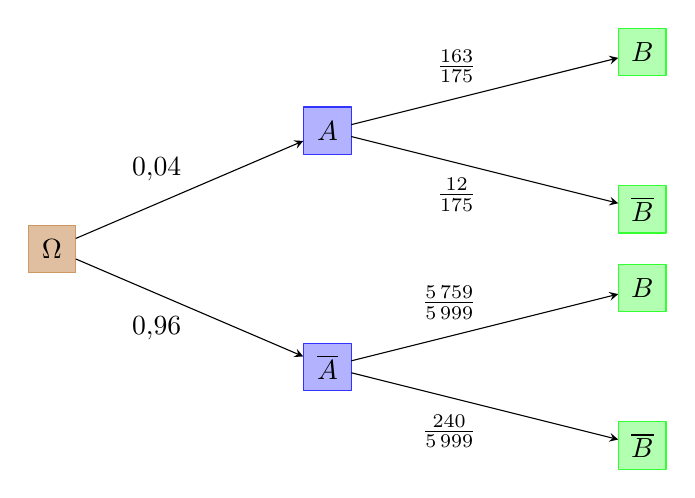
\begin{tikzpicture}[
				line join = round,line cap = round,>=stealth,scale=1,inner sep = 1mm,
				hcnxanh/.style={rectangle,draw = blue!80,fill = blue!30, minimum width=0.6cm, minimum height=0.6cm},
				hcng/.style={rectangle,draw = green!80,fill = green!30, minimum width=0.6cm, minimum height=0.6cm},
				hcnnau/.style={rectangle,draw = brown!80,fill = brown!50, minimum width=0.6cm, minimum height=0.6cm}]
				\node at (0,0) (nodeO) [hcnnau] {$\Omega$};
				\node at (3.5,1.5) (nodeA) [hcnxanh] {$A$};
				\node at (3.5,-1.5) (nodeAd) [hcnxanh] {$\overline{A}$};
				\node at (7.5,2.5) (nodeB1) [hcng] {$B$};
				\node at (7.5,0.5) (nodeB2) [hcng] {$\overline{B}$};
				\node at (7.5,-0.5) (nodeB3) [hcng] {$B$};
				\node at (7.5,-2.5) (nodeB4) [hcng] {$\overline{B}$};
				\draw[->] (nodeO) to node[above left]{$0{,}04$} (nodeA);
				\draw[->] (nodeO) to node[below left]{$0{,}96$} (nodeAd);
				\draw[->] (nodeA) to node[above left]{$\frac{163}{175}$} (nodeB1);
				\draw[->] (nodeA) to node[below left]{$\frac{12}{175}$} (nodeB2);
				\draw[->] (nodeAd) to node[above left]{$\frac{5\,759}{5\,999}$} (nodeB3);
				\draw[->] (nodeAd) to node[below left]{$\frac{240}{5\,999}$} (nodeB4);
			\end{tikzpicture}
		\end{center}
		Áp dụng công thức xác suất toàn phần, xác suất lần hai chọn được áo tốt là
		\[\mathrm{P}(B) = \mathrm{P}(A)\mathrm{P}(B \mid A) + \mathrm{P}\left(\overline{A}\right)\mathrm{P}\left(B \mid \overline{A}\right) = 0{,}04 \cdot \dfrac{163}{175} + 0{,}96 \cdot \dfrac{5\,759}{5\,999} = \dfrac{3\,595\,091}{3\,749\,375}.\]
		Áp dụng công thức Bayes, xác suất lần một chọn được áo phế phẩm biết rằng lần hai chọn được áo tốt là
		\[\mathrm{P}(A \mid B) = \dfrac{\mathrm{P}(A)\mathrm{P}(B \mid A)}{\mathrm{P}(B)} = \dfrac{0{,}04 \cdot \dfrac{163}{175}}{\dfrac{3\,595\,091}{3\,749\,375}} = \dfrac{139\,691}{3\,595\,091} \approx 0{,}04.\]
		Vậy xác suất cần tìm là $0{,}04$.
	}
\end{ex}
%%%=============================%%%

%%%=============EX_20=============%%%
\begin{ex}%[2D4C3-5]%[TDM32]%[Nguyễn Văn Sang]
	\immini[thm]{Cho ba hình phẳng $(H_1)$, $(H_2)$, $(H_3)$ được tô màu như hình vẽ bên dưới, tạo ra bởi một đường tròn $(C)$ có bán kính bằng $30$\,cm và một elip $(E)$ nhận hai điểm $A$ và $B$ là hai tiêu điểm với $AB$ là đường kính của $(C)$, biết rằng elip $(E)$ có trục dài là $72$\,cm. Tiến hành sơn màu một mặt cho $(H_1)$, $(H_2)$, $(H_3)$ các loại sơn có giá tương ứng là $100$\,đồng/cm$^2$, $120$\,đồng/cm$^2$, $150$\,đồng/cm$^2$. Hãy tính theo đơn vị nghìn đồng chi phí dùng để sơn (\textit{làm tròn kết quả đến hàng đơn vị}).}{
		\begin{tikzpicture}[scale=0.1,font=\footnotesize,line join=round,line cap=round]
			\begin{scope}
				\clip (0,0) circle (25);
				\fill[pattern=dots,pattern color=blue!50] (0,0) circle (25);
				\fill[white] (0,0) ellipse (35 and 15);
			\end{scope}
			\begin{scope}
				\clip (0,0) ellipse (35 and 15);
				\fill[pattern=grid,pattern color=green!60!black] (0,0) ellipse (35 and 15);
				\fill[white] (0,0) circle (25);
			\end{scope}
			\begin{scope}
				\clip (0,0) circle (25);
				\clip (0,0) ellipse (35 and 15);
				\fill[pattern=north east lines,pattern color=red!70] (-40,-40) rectangle (40,40);
			\end{scope}
			\draw[blue] (0,0) circle (25) node[above=25pt] {$(C)$};
			\draw[red] (0,0) ellipse (35 and 15) node[below right=28pt] {$(E)$};
			\node at (0,20) {$(H_1)$};
			\node at (0,-20) {$(H_1)$};
			\node at (30,0) {$(H_2)$};
			\node at (-30,0) {$(H_2)$};
			\node at (0,0) [fill=white,inner sep=1pt,opacity=0.8,text opacity=1] {$(H_3)$};
			\draw[dashed,gray] (-35,0) -- (-35,-28);
			\draw[dashed,gray] (35,0) -- (35,-28);
			\draw[<->,>=stealth] (-35,-28) -- (35,-28) node[midway,fill=white] {$72$\,cm};
		\end{tikzpicture}
	}
	\par
	\shortans[0]{411}
	\loigiai{
		Chọn hệ trục tọa độ $Oxy$ với $O$ là tâm của đường tròn và elip.
		\begin{center}
			\begin{tikzpicture}[scale=0.1,font=\footnotesize,>=stealth]
				\draw[->] (-45,0) -- (45,0) node[below] {$x$};
				\draw[->] (0,-35) -- (0,35) node[left] {$y$};
				\node[below left] at (0,0) {$O$};
				\draw[blue] (0,0) circle (30);
				\draw[red] (0,0) ellipse (36 and 19.9);
				\filldraw[] (-30,0) circle (1.5pt) node[below left] {$A(-30; 0)$};
				\filldraw[] (30,0) circle (1.5pt) node[below right] {$B(30; 0)$};
				\filldraw[] (36,0) circle (1.5pt) node[above right] {$36$};
				\filldraw[] (0,19.9) circle (1.5pt) node[above left] {$\sqrt{396}$};
				\filldraw[purple] ({36*sqrt(14)/5}, 13.2) circle (1.5pt) node[above right] {$E\left(\dfrac{36\sqrt{14}}{5}; 13{,}2\right)$};
				\draw[dashed,gray] ({36*sqrt(14)/5},0) -- ({36*sqrt(14)/5}, 13.2) -- (0,13.2);
				\node[above, blue] at (22,22) {$(C)$};
				\node[red] at (38,10) {$(E)$};
			\end{tikzpicture}
		\end{center}
		Đường tròn $(C)$ có tâm $O$, bán kính $R = 30$ nên có phương trình $(C)\colon x^2 + y^2 = 900$.\\
		Diện tích hình tròn là $S_{(C)} = \pi R^2 = 900\pi$\,(cm$^2$).\\
		Elip $(E)$ có trục dài $2a = 72 \Rightarrow a = 36$.\\
		Vì hai tiêu điểm $A$, $B$ thuộc đường kính của $(C)$ nên tiêu cự $2c = 2R = 60 \Rightarrow c = 30$.\\
		Ta có $b^2 = a^2 - c^2 = 36^2 - 30^2 = 396$.\\
		Phương trình chính tắc của elip là $(E)\colon \dfrac{x^2}{1\,296} + \dfrac{y^2}{396} = 1$.\\
		Diện tích elip là $S_{(E)} = \pi ab = \pi \cdot 36 \cdot \sqrt{396} = 216\pi\sqrt{11}$\,(cm$^2$).\\
		Hoành độ giao điểm của $(C)$ và $(E)$ là nghiệm của hệ phương trình
		\[\heva{&x^2 + y^2 = 900 \\ &\dfrac{x^2}{1\,296} + \dfrac{y^2}{396} = 1} \Leftrightarrow \heva{&x^2 = \dfrac{18\,144}{25} \\ &y^2 = \dfrac{4\,356}{25}} \Rightarrow \hoac{&x=\dfrac{36\sqrt{14}}{5}\\&x=-\dfrac{36\sqrt{14}}{5}.} \]
		Do tính đối xứng, diện tích hình $(H_1)$ bằng $4$ lần diện tích phần hình $(H_1)$ nằm ở góc phần tư thứ nhất (giới hạn bởi nửa trên đường tròn $(C)\colon y = \sqrt{900 - x^2}$ và nửa trên elip $(E)\colon y = \sqrt{396\left(1 - \dfrac{x^2}{1\,296}\right)}$).\\
		Diện tích hình $(H_1)$ được thiết lập bằng công thức tích phân
		\[S_{H_1} = 4 \displaystyle\int\limits_0^{\frac{36\sqrt{14}}{5}} \left[\sqrt{900 - x^2} - \sqrt{396\left(1 - \dfrac{x^2}{1\,296}\right)} \right] \mathrm{\,d}x. \]
		Hình tròn $(C)$ được chia thành hai phần là $(H_1)$ và $(H_3)$ nên ta có
		\[S_{H_3} = S_{(C)} - S_{H_1} = 900\pi - S_{H_1}. \]
		Tương tự, hình elip $(E)$ được chia thành phần $(H_2)$ và $(H_3)$ nên ta có
		\[S_{H_2} = S_{(E)} - S_{H_3} = 216\pi\sqrt{11} - \left(900\pi - S_{H_1}\right) = 216\pi\sqrt{11} - 900\pi + S_{H_1}. \]
		Tổng chi phí sơn $T$ (đồng) là
		\allowdisplaybreaks
		\begin{align*}
			T &= 100 \cdot S_{H_1} + 120 \cdot S_{H_2} + 150 \cdot S_{H_3} \\
			&= 100 \cdot S_{H_1} + 120 \left(216\pi\sqrt{11} - 900\pi + S_{H_1} \right) + 150 \left(900\pi - S_{H_1} \right) \\
			&= 70 \cdot S_{H_1} + 25\,920\pi\sqrt{11} + 27\,000\pi \\
			&= 70 \cdot 4 \int\limits_0^{\frac{36\sqrt{14}}{5}} \left[\sqrt{900 - x^2} - \sqrt{396\left(1 - \dfrac{x^2}{1\,296}\right)} \right] \mathrm{\,d}x + 25\,920\pi\sqrt{11} + 27\,000\pi \\
			&\approx 410\,705{,}36 \text{ (đồng)}.
		\end{align*}
		Làm tròn kết quả đến hàng đơn vị theo đơn vị nghìn đồng, chi phí cần thiết là $411$ nghìn đồng.
	}
\end{ex}
%%%=============================%%%

%%%=============EX_21=============%%%
\begin{ex}%[2H5V2-8]%[TDMT14]%[Lê Hồ Quang Minh]
	Khi gắn hệ toạ độ $Oxyz$ vào thì ta có toạ độ của một nguồn sáng điểm là $S(3;7;-2)$ và hai gương phẳng là hai mặt phẳng có hai mặt phản xạ quay vào nhau tạo góc nhọn có phương trình lần lượt là $(\alpha) \colon z = 0$ và $(\beta) \colon y + z = 0$. Một tia sáng đi từ $S$ sau khi lần lượt phản xạ (tia sáng bị bật trở lại) qua gương $(\alpha)$ và gương $(\beta)$ thì đến điểm $A(3;6;-5)$. \textbf{Biết rằng tia sáng rất là thông minh nó luôn tìm con đường đi là ngắn nhất để đi}. Hãy xác định độ dài đường đi của tia sáng này (\textit{làm tròn kết quả đến hàng phần trăm}).
	\par 
	\shortans[0]{8,25}
	\loigiai{
		\begin{center}
			\begin{minipage}{0.48\textwidth}
				\centering
				\begin{tikzpicture}[x={(-0.5cm,-0.4cm)}, y={(1cm,0cm)}, z={(0cm,1cm)}, scale=0.8, >=stealth, line join=round, line cap=round, font=\scriptsize]
					\draw[->] (0,0,0) -- (6,0,0) node[below] {$x$};
					\draw[->] (0,-1,0) -- (0,9,0) node[right] {$y$};
					\draw[->] (0,0,-7) -- (0,0,4) node[above] {$z$};
					\draw[fill=blue!10, opacity=0.7] (0,0,0) -- (5,0,0) -- (5,8.5,0) -- (0,8.5,0) -- cycle;
					\node[blue] at (3, 9.25, 1) {$(\alpha)$};
					\draw[fill=red!10, opacity=0.7] (0,0,0) -- (5,0,0) -- (5,6.5,-6.5) -- (0,6.5,-6.5) -- cycle;
					\node[red] at (2, 7, -5.75) {$(\beta)$};
					\coordinate (S) at (3,7,-2);
					\coordinate (Sp) at (3,7,2);
					\coordinate (A) at (3,6,-5);
					\coordinate (Ap) at (3,5,-6);
					\coordinate (M) at (3,6.5,0);
					\coordinate (N) at (3,5.2,-5.2);
					\coordinate (H) at (3,5.5,-5.5);
					\draw[dashed, gray] (3,0,0) -- (3,8,0);
					\draw[dashed, gray] (3,0,0) -- (3,7,-7);
					\draw[dashed] (S) -- (Sp) (A) -- (Ap);
					\draw[dashed, blue] (Sp) -- (M) (N) -- (Ap);
					\draw[thick, red, ->] (S) -- (M);
					\draw[thick, red, ->] (M) -- (N);
					\draw[thick, red, ->] (N) -- (A);
					\foreach \p in {S, Sp, A, Ap, M, N, H} {
						\fill (\p) circle (1.5pt);
					}
					\node[right] at (S) {$S$};
					\node[above right] at (Sp) {$S'$};
					\node[above] at (A) {$A$};
					\node[below right] at (Ap) {$A'$};
					\node[above left] at (M) {$M$};
					\node[below left] at (N) {$N$};
					\node[right] at (H) {$H$};
					\node[above=0.2cm] at (2.5,9,3) {\textbf{Minh họa 3D}};
				\end{tikzpicture}
			\end{minipage}\hfill
			\begin{minipage}{0.48\textwidth}
				\centering
				\begin{tikzpicture}[>=stealth,line join=round,line cap=round,scale=0.8,every node/.style={font=\scriptsize},
					declare function={
						xmin = 0; xmax = 8.5;
						ymin = -6.5; ymax = 3;
						yS=7; zS=-2;
						ySp=7; zSp=2;
						yA=6; zA=-5;
						yAp=5; zAp=-6;
						yM=6.5; zM=0;
						yN=5.2; zN=-5.2;
						yH=5.5; zH=-5.5;
					}]
					\draw[dashed,-stealth] (xmin,0) -- (xmax,0) node[below,font=\scriptsize] {$y$};
					\draw[-stealth] (0,ymin) -- (0,ymax) node[left,font=\scriptsize] {$z$};
					\path
					(0,0) coordinate (O)
					(yS,zS) coordinate (S)
					(ySp,zSp) coordinate (Sp)
					(yA,zA) coordinate (A)
					(yAp,zAp) coordinate (Ap)
					(yM,zM) coordinate (M)
					(yN,zN) coordinate (N)
					(yH,zH) coordinate (H);
					\draw[red,thick] (O) -- (7.5,0) node[pos=0.4,sloped,above,font=\scriptsize] {$(\alpha)$};
					\draw[red,thick] (O) -- (6.5,-6.5) node[pos=0.5,sloped,above,font=\scriptsize] {$(\beta)$};
					\draw[dashed] (S) -- (Sp)
					(A) -- (Ap);
					\draw[dashed] (Sp) -- (M)
					(N) -- (Ap);
					\draw (S) -- (M) -- (N) -- (A);
					\foreach \p/\pos/\dist/\lab in {
						O/180/10/O,
						S/-30/16/{S(3; 7; -2)},
						Sp/30/16/{S'(3; 7; 2)},
						A/30/16/{A(3; 6; -5)},
						Ap/-30/16/{A'(3; 5; -6)},
						M/-135/10/M,
						N/170/10/N,
						H/0/10/H
					}{
						\fill (\p) circle (1pt) node[shift={(\pos:\dist pt)},font=\scriptsize] {$\lab$};
					}
					\node[above=0.2cm] at (4,3) {\textbf{Chiếu trên mặt phẳng } $x=3$};
				\end{tikzpicture}
			\end{minipage}
		\end{center}
		Ta dễ dàng nhận ra hai gương $(\alpha)$ và $(\beta)$ giao nhau theo trục $Ox$ (do hệ phương trình $z=0$ và $y+z=0$ cho ta $y=0$, $z=0$).\\
		Hai điểm $S(3;7;-2)$ và $A(3;6;-5)$ có cùng hoành độ $x=3$, nên chúng cùng nằm trong mặt phẳng $x=3$ vuông góc với trục $Ox$.\\
		Do đó, ta có thể biểu diễn hình học của bài toán trên mặt phẳng tọa độ $Oyz$ (cắt bởi mặt phẳng $x=3$) như hình vẽ.\\	
		Gọi $M \in (\alpha)$ và $N \in (\beta)$ lần lượt là các điểm phản xạ của tia sáng.\\
		Độ dài đường đi của tia sáng là $L = SM + MN + NA$.\\
		Gọi $S'$ là điểm đối xứng với $S(3;7;-2)$ qua $(\alpha) \colon z=0$.\\
		Suy ra $S'(3; 7; 2)$.\\
		Gọi $A'$ là điểm đối xứng của $A(3;6;-5)$ qua mặt phẳng $(\beta) \colon y+z=0$.\\
		Đường thẳng qua $A$ vuông góc với $(\beta)$ có phương trình là $\Delta \colon \heva{&x=3 \\ &y=6+t \\ &z=-5+t.}$\\
		Gọi $H$ là giao điểm của $\Delta$ và $(\beta)$.\\ Thay tọa độ vào phương trình $(\beta)$ ta được
		\[6+t + (-5+t) = 0 \Leftrightarrow 2t+1 = 0 \Leftrightarrow t = -0{,}5.\]
		Suy ra tọa độ điểm $H(3; 5{,}5; -5{,}5)$.\\
		Vì $H$ là trung điểm của $AA'$ nên tọa độ $A'$ là
		\[\heva{&x_{A'} = 2x_H - x_A = 2 \cdot 3 - 3 = 3 \\ &y_{A'} = 2y_H - y_A = 2 \cdot 5{,}5 - 6 = 5 \\ &z_{A'} = 2z_H - z_A = 2 \cdot (-5{,}5) - (-5) = -6} \Rightarrow A'(3; 5; -6).\]
		Dựa vào tính chất đối xứng của gương phẳng, ta có $SM = S'M$ và $NA = NA'$.\\
		Khi đó, độ dài đường đi của tia sáng là
		\[L = SM + MN + NA = S'M + MN + NA' \ge S'A'.\]
		Đường đi của tia sáng ngắn nhất khi $4$ điểm $S'$, $M$, $N$, $A'$ thẳng hàng, khi đó giá trị nhỏ nhất của $L$ chính là độ dài đoạn thẳng $S'A'$.\\
		Ta có
		\[S'A' = \sqrt{(3-3)^2 + (5 - 7)^2 + (-6 - 2)^2} = \sqrt{0^2 + (-2)^2 + (-8)^2} = \sqrt{68} = 2\sqrt{17} \approx 8{,}246.\]
		Vậy độ dài đường đi ngắn nhất của tia sáng làm tròn đến hàng phần trăm là $8{,}25$.
	}
\end{ex}
%%%=============================%%%

%%%=============EX_22=============%%%
\begin{ex}%[0D0C2-3]%[TDMT14]%[Nguyễn Thành Hậu]
	\immini[thm]{Cho $5$ ô vuông $a$, $b$, $c$, $d$, $e$ được bố trí như hình vẽ bên dưới.
		Biết rằng có tất cả $T$ cách chọn ra $5$ số nguyên khác nhau từ tập $X=\{1,2,\ldots 13\}$ để xếp vào $5$ ô vuông $a$, $b$, $c$, $d$, $e$
		sao cho mỗi ô vuông nhỏ chỉ xếp được đúng một số và các ô hàng ngang được sắp xếp theo thứ tự tăng dần hoặc giảm dần,
		còn các ô hàng dọc thì không được sắp xếp theo thứ tự tăng dần hoặc giảm dần.
		Hãy xác định $\dfrac{T}{10}$ (\textit{làm tròn kết quả đến hàng đơn vị}).}{
		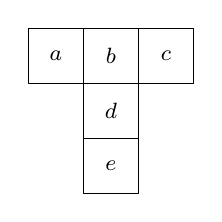
\begin{tikzpicture}[line cap=round,line join=round,>=stealth,font=\footnotesize,scale=1]
			\def\s{0.7cm}
			\draw (0,0) rectangle (\s,\s) node[pos=.5] {$a$};
			\draw (\s,0) rectangle (2*\s,\s) node[pos=.5] {$b$};
			\draw (2*\s,0) rectangle (3*\s,\s) node[pos=.5] {$c$};
			\draw (\s,-\s) rectangle (2*\s,0) node[pos=.5] {$d$};
			\draw (\s,-2*\s) rectangle (2*\s,-\s) node[pos=.5] {$e$};
		\end{tikzpicture}
	}
	\par
	\shortans[0]{3604}
	\loigiai{
		Chọn $5$ số bất kỳ từ tập $X$ gồm $13$ phần tử, ta có $\mathrm{C}_{13}^{5}$ cách chọn.\\
		Giả sử $5$ số được chọn sắp xếp theo thứ tự tăng dần là $x_1 < x_2 < x_3 < x_4 < x_5$.\\
		\textbf{Cách 1: Đếm trực tiếp (chia trường hợp theo vị trí ô trung tâm).}\\
		Vì $3$ ô hàng ngang $a$, $b$, $c$ phải xếp tăng dần hoặc giảm dần nên ô trung tâm $b$ không thể chứa số nhỏ nhất ($x_1$) hoặc số lớn nhất ($x_5$).\\ Do đó, $b \in \{x_2; x_3; x_4\}$. \\
		Ta chia làm $3$ trường hợp áp dụng quy tắc cộng
		\begin{center}
			\begin{tikzpicture}[>=stealth,line width=0.8pt,scale=1,font=\footnotesize]
				\foreach \i in {1,2,3,4,5}{
					\node[draw,circle,inner sep=1pt,minimum size=0.6cm,fill=cyan!10] (x\i) at (\i*2.5,0) {\color{blue}$x_\i$};
				}
				\draw[->,blue!70] (x2) -- ++(0,-1.8) node[midway,left] {Chọn $b$}
				node[below,align=center] {Ngang: $\color{blue}2 \times \mathrm{C}_3^1$ \\ Dọc: $\color{blue}1$ \\ $\Rightarrow \color{blue}6$ cách};
				\draw[->,red!70] (x3) -- ++(0,-3) node[midway,right] {Chọn $b$}
				node[below,align=center] {Ngang: $\color{blue}2 \times \mathrm{C}_2^1 \cdot \mathrm{C}_2^1$ \\ Dọc: $\color{blue}2!$ \\ $\Rightarrow \color{blue}16$ cách};
				\draw[->,blue!70] (x4) -- ++(0,-1.8) node[midway,right] {Chọn $b$}
				node[below,align=center] {Ngang: $\color{blue}2 \times \mathrm{C}_3^1$ \\ Dọc: $\color{blue}1$ \\ $\Rightarrow \color{blue}6$ cách};
			\end{tikzpicture}
		\end{center}
		\begin{itemize}
			\item \textbf{Trường hợp 1: $b = x_2$.}
			\begin{itemize}
				\item \textit{Xếp hàng ngang ($a$, $c$):}\\
				Để tạo thành dãy đơn điệu, một bên của $b$ phải là $x_1$, bên còn lại chọn $1$ số từ $\{x_3; x_4; x_5\}$ (có $\mathrm{C}_3^1 = 3$ cách).\\ Có $2$ cách đảo vị trí $a$, $c$ (để tạo dãy tăng hoặc giảm).\\ Suy ra có $1 \times 3 \times 2 = 6$ cách xếp hàng ngang.
				\item \textit{Xếp hàng dọc ($d$, $e$):}\\ Hai số còn lại đều lớn hơn $x_2$.\\ Gọi hai số đó là $u < v$.\\ Dãy dọc $b$, $d$, $e$ tương ứng là $x_2$, $d$, $e$.\\ Để dãy dọc \textbf{không} tăng/giảm (mà $x_2$ đã là nhỏ nhất), ta bắt buộc phải xếp số lớn hơn vào $d$ và số nhỏ hơn vào $e$ (tức là $x_2 < v > u$).\\ Do đó, chỉ có $1$ cách xếp hàng dọc.
			\end{itemize}
			Theo quy tắc nhân, trường hợp $1$ có $6 \times 1 = 6$ cách.
			\item \textbf{Trường hợp 2: $b = x_3$.}
			\begin{itemize}
				\item \textit{Xếp hàng ngang ($a$, $c$):} Một bên của $b$ chọn từ $\{x_1; x_2\}$ (có $\mathrm{C}_2^1 = 2$ cách), bên còn lại chọn từ $\{x_4; x_5\}$ (có $\mathrm{C}_2^1 = 2$ cách).\\ Đảo vị trí $a$, $c$ có $2$ cách.\\ Số cách xếp là $2 \times 2 \times 2 = 8$ cách.
				\item \textit{Xếp hàng dọc ($d$, $e$):} Hai số còn lại chắc chắn có một số nhỏ hơn $x_3$ và một số lớn hơn $x_3$.\\ Vì $b=x_3$ nằm giữa giá trị của hai số này, nên dù ta xếp $d$, $e$ kiểu gì thì hàng dọc $b$, $d$, $e$ cũng sẽ đổi chiều (tăng rồi giảm, hoặc giảm rồi tăng), \textbf{luôn thỏa mãn} điều kiện không đơn điệu.\\ Số cách xếp tự do $2$ số vào $d$, $e$ là $2! = 2$ cách.
			\end{itemize}
			Theo quy tắc nhân, trường hợp $2$ có $8 \times 2 = 16$ cách.
			\item \textbf{Trường hợp 3: $b = x_4$.}
			Do tính đối xứng với trường hợp $1$, ta dễ dàng suy ra có $6$ cách xếp thỏa mãn.
		\end{itemize}
		Áp dụng quy tắc nhân cho cả quá trình, tổng số cách xếp là
		\[T = \mathrm{C}_{13}^{5} \cdot (6 + 16 + 6) = 1\,287 \cdot 28 = 36\,036 \text{ (cách)}.\]
		\noindent \textbf{Cách 2: Sử dụng biến cố phần bù}\\
		Gọi $A$ là tập hợp các cách xếp sao cho hàng ngang ($a$, $b$, $c$) đơn điệu (tăng hoặc giảm).\\
		Gọi $B$ là tập hợp các cách xếp sao cho hàng dọc ($b$, $d$, $e$) \textbf{không} đơn điệu.\\
		Tập hợp các cách xếp thỏa mãn yêu cầu bài toán là $A \cap B$. Ta có
		\[n(A \cap B) = n(A) - n\left(A \cap \overline{B}\right)\]
		\begin{itemize}
			\item \textbf{Tính $n(A)$ (chỉ quan tâm hàng ngang đơn điệu):}\\
			Để xếp $5$ số sao cho hàng ngang đơn điệu
			\begin{itemize}
				\item Chọn $3$ số từ $5$ số để xếp vào $a$, $b$, $c$ có $\mathrm{C}_5^3 = 10$ cách.
				\item Xếp $3$ số này theo thứ tự tăng dần hoặc giảm dần có $2$ cách.
				\item Hai số còn lại xếp vào $d$, $e$ có $2! = 2$ cách.
			\end{itemize}
			Theo quy tắc nhân, với mỗi bộ $5$ số có $10 \cdot 2 \cdot 2 = 40$ cách xếp. \\
			Suy ra $n(A) = 40 \cdot \mathrm{C}_{13}^5 = 51\,480$.
			\item \textbf{Tính $n\left(A \cap \overline{B}\right)$ (Cả hàng ngang và hàng dọc đều đơn điệu):}\\
			Vì hàng ngang đơn điệu nên $b$ nằm giữa giá trị của $a$ và $c$. \\
			Vì hàng dọc đơn điệu ($b$, $d$, $e$) nên $b$ phải nhỏ hơn cả $d$, $e$ hoặc lớn hơn cả $d$, $e$.\\
			Suy ra trong $5$ số, $b$ phải có đúng $1$ số nhỏ hơn và $3$ số lớn hơn (tức $b = x_2$), hoặc có đúng $3$ số nhỏ hơn và $1$ số lớn hơn (tức $b = x_4$).
			\begin{itemize}
				\item \textit{Nếu $b = x_2$:} Hàng ngang bắt buộc dùng số $x_1$ và $1$ số từ $\{x_3; x_4; x_5\}$ (có $\mathrm{C}_3^1 = 3$ cách).\\ Đảo vị trí ngang có $2$ cách.\\ Hàng dọc dùng $2$ số còn lại, vì cả hai đều lớn hơn $x_2$ nên để dọc đơn điệu chỉ có $1$ cách xếp tăng dần ($x_2 < d < e$).\\ Số cách xếp là $3 \cdot 2 \cdot 1 = 6$ cách.
				\item \textit{Nếu $b = x_4$:} Tương tự, có $6$ cách xếp.
			\end{itemize}
			Tổng cộng với mỗi bộ $5$ số có $6 + 6 = 12$ cách xếp cả ngang và dọc đều đơn điệu. \\
			Suy ra $n\left(A \cap \overline{B}\right) = 12 \cdot \mathrm{C}_{13}^5 = 15\,444$.
		\end{itemize}
		Tổng số cách xếp thỏa mãn bài toán là
		\[T = n(A \cap B) = 51\,480 - 15\,444 = 36\,036 \text{ (cách)}.\]
		Vậy $\dfrac{T}{10} = \dfrac{36\,036}{10} = 3\,603{,}6 \approx 3\,604$.
	}
\end{ex}
%%%=============================%%%
\Closesolutionfile{ans}

\newpage
\indapan{12}{ans/ansTN-Dung}
\indapan[TF]{2}{ans/ansTN-DungSai}
\indapan[SA]{6}{ans/ansTN-DienKhuyet}
%%%%%%%%%%%%%%
%%nhãn kết thúc đề (để đếm số trang tự động mỗi đề)
\label{B\thedeso}